\chapter{Design}

% Containing a comprehensive description of the design chosen, how it addresses the problem, and why it is designed the way it is.

\section{Architectural Model}

Architectural design decisions for this project have been heavily influenced by the requirement that the system should be federated, not relying on any individual provider. A number of possible architectural models were proposed as outlined below.

\begin{enumerate}
  \item \label{itm:web-cloud} A web based system, hosted on a cloud service provider such as Amazon Web Services (AWS), Google Cloud Platform (GCP) or Microsoft Azure.
  \item \label{itm:on-demand-cloud} A locally installed application which spins up a compute instance on a cloud service provider on demand for each user for handling computationally expensive work.
  \item \label{itm:local-service} A locally running web-based user interface which communicates with a separate locally running service process.
  \item \label{itm:electron} An Electron application which encapsulates the frontend and backend service into a single executable that can be run locally.
\end{enumerate}

Each of the models listed above present their own advantages and disadvantages. Although \ref{itm:web-cloud} would mean that the software is accessible from anywhere, by any device with a web browser, it also means that users have no choice but to trust the backend of this software, running in the cloud, with their data, which means that the federated aspect of the system is lost.

In \ref{itm:on-demand-cloud}, users would have more control over their data in the cloud, as they are responsible for managing the compute instance, however implementing this model would mean that users are required to have in-depth knowledge of AWS or similar, which detracts from the usability of the system.

The model proposed in \ref{itm:local-service} does not rely on any remotely hosted software, and so maintains the integrity of the federated system. Furthermore, by keeping the service as a separate entity, it would be relatively simple to access it from other devices, for example a mobile phone on the same network as the host PC, using a consistent API. However, by requiring users to manually start the user interface, navigate to it in the browser, and then start the service, it increases the barrier to entry for less technical users.

The Electron application proposed in \ref{itm:electron} will be easy for users to set up and run since it will consist of running a single executable, and it allows for web technologies to be used to build a desktop application. A disadvantage of using this model is that the application will only be available on desktop devices.

It is clear that the final solution will require compromises, and that any architecture will have flaws. It was decided that the most important requirements that the system architecture should fulfill are ease of use, to ensure that the software is accessible to as many users as possible, and that the system should be entirely federated. Therefore, the most suitable architectural model, and the one to be used in this project is \ref{itm:electron}, despite the fact that this limits the platform to desktops only.

\section{Message Threading Model}
An important design aspect of this project is deciding on a suitable message threading model to maximise functionality and usability. Indeed, one of the motivations for completing this project is that email as used in its present form does not handle complex thread structures well. The need for message threading stems from the requirement that users are able to directly reply to messages. In designing this system, it was noted that current messaging software products use various different models for message threading, and that the possible models must be evaluated in order to ascertain the most appropriate for this project.

There is a considerable amount of previous work on how best to handle message threading, particularly within the scope of email. Lewis \& Knowles stated that: ``While user clients typically insert in messages structural information useful for recovering threads, inconsistencies between clients, loose standards, creative user behavior, and the subjective nature of conversation make threading systems based on structural information only partially successful.'' \cite{lewis1997threading}. This project aims to avoid the issues of client inconsistencies and loose standards by providing a specialised client application and well-defined data structure to be sent using email as a transport mechanism.

It is important to realise that one message can have multiple replies, each initiating a separate message thread. For this reason, message threads are best modeled using a tree structure \cite{palme1998message}. In email, there does not exist an explicit reference from a message to its replies, so the relationship can be described as unidirectional from reply to parent. Some email clients provide a feature to generate these reverse links, which are useful to allow a user to see if replies already exist before composing their own \cite{palme1998message}, though this functionality is by no means universal. Outside of email, there is a mix of bidirectional and unidirectional relationships between replies and their parents.

In order to pick a threading system for this project, a review of several popular existing social messaging applications was conducted, highlighting the advantages and disadvantages of their threading models. The results of this research are summarised below.

\begin{itemize}
  \item Slack Model
    \begin{itemize}
      \item A message provides links to its replies.
      \item Only one level of replies is allowed. Replies cannot be replied to.
      \item Replies can only be accessed via their parent message.
    \end{itemize}
  \item Twitter Model
    \begin{itemize}
      \item Replies can be traced back to the parent from any level, and parent has links to all direct and indirect replies.
      \item Replies can be replied to up to an infinite depth.
    \end{itemize}
  \item Facebook Messenger Model
    \begin{itemize}
      \item Replies can be traced back to the parent from any depth, but a parent message does not provide any links to its replies.
      \item Replies can be replied to up to an infinite depth.
    \end{itemize}
\end{itemize}

It is interesting to note that during development, the message threading model used by Slack went through many different iterations involving both conceptual structure and user interface design \cite{florin2018}. This research at Slack found that when users were allowed to reply to replies, threads quickly became very complex and difficult for users to understand, leading to the approach currently implemented in Slack where each thread is restricted to one level of replies \cite{florin2018}.

The final design decision is a tradeoff between functionality and usability. Whilst allowing greater depth of replies provides users with more flexibility in the way that they construct conversations, it also detracts from usability, with it becoming more difficult for users to follow the discussions that they are interested in. It is proposed that this project will initially implement a threading structure similar to that of Slack, with replies limited to one level deep. Following this implementation, User Testing will be conducted to ascertain whether this model allows enough flexibility for users to hold discussions, whilst being easy to use. If the results of this testing indicate a need for more complex threading then the design will be revisited.

\section{User Interface}

An important element of this project is to create a simple and intuitive user interface. Some elements of the interface that were decided as essential are as follows:
\begin{itemize}
  \item Facility to enter email account credentials
  \item `New Conversation' button
  \item List of conversations
  \item Ability to view messages and their replies
  \item Sender Indicators
  \item Composer
  \item `Add Attachment' button
\end{itemize}

Based on these UI elements, wireframes were produced, seen in figures \ref{fig:sketch-main}, \ref{fig:sketch-login}.

\begin{figure}[h!]
  \centering
  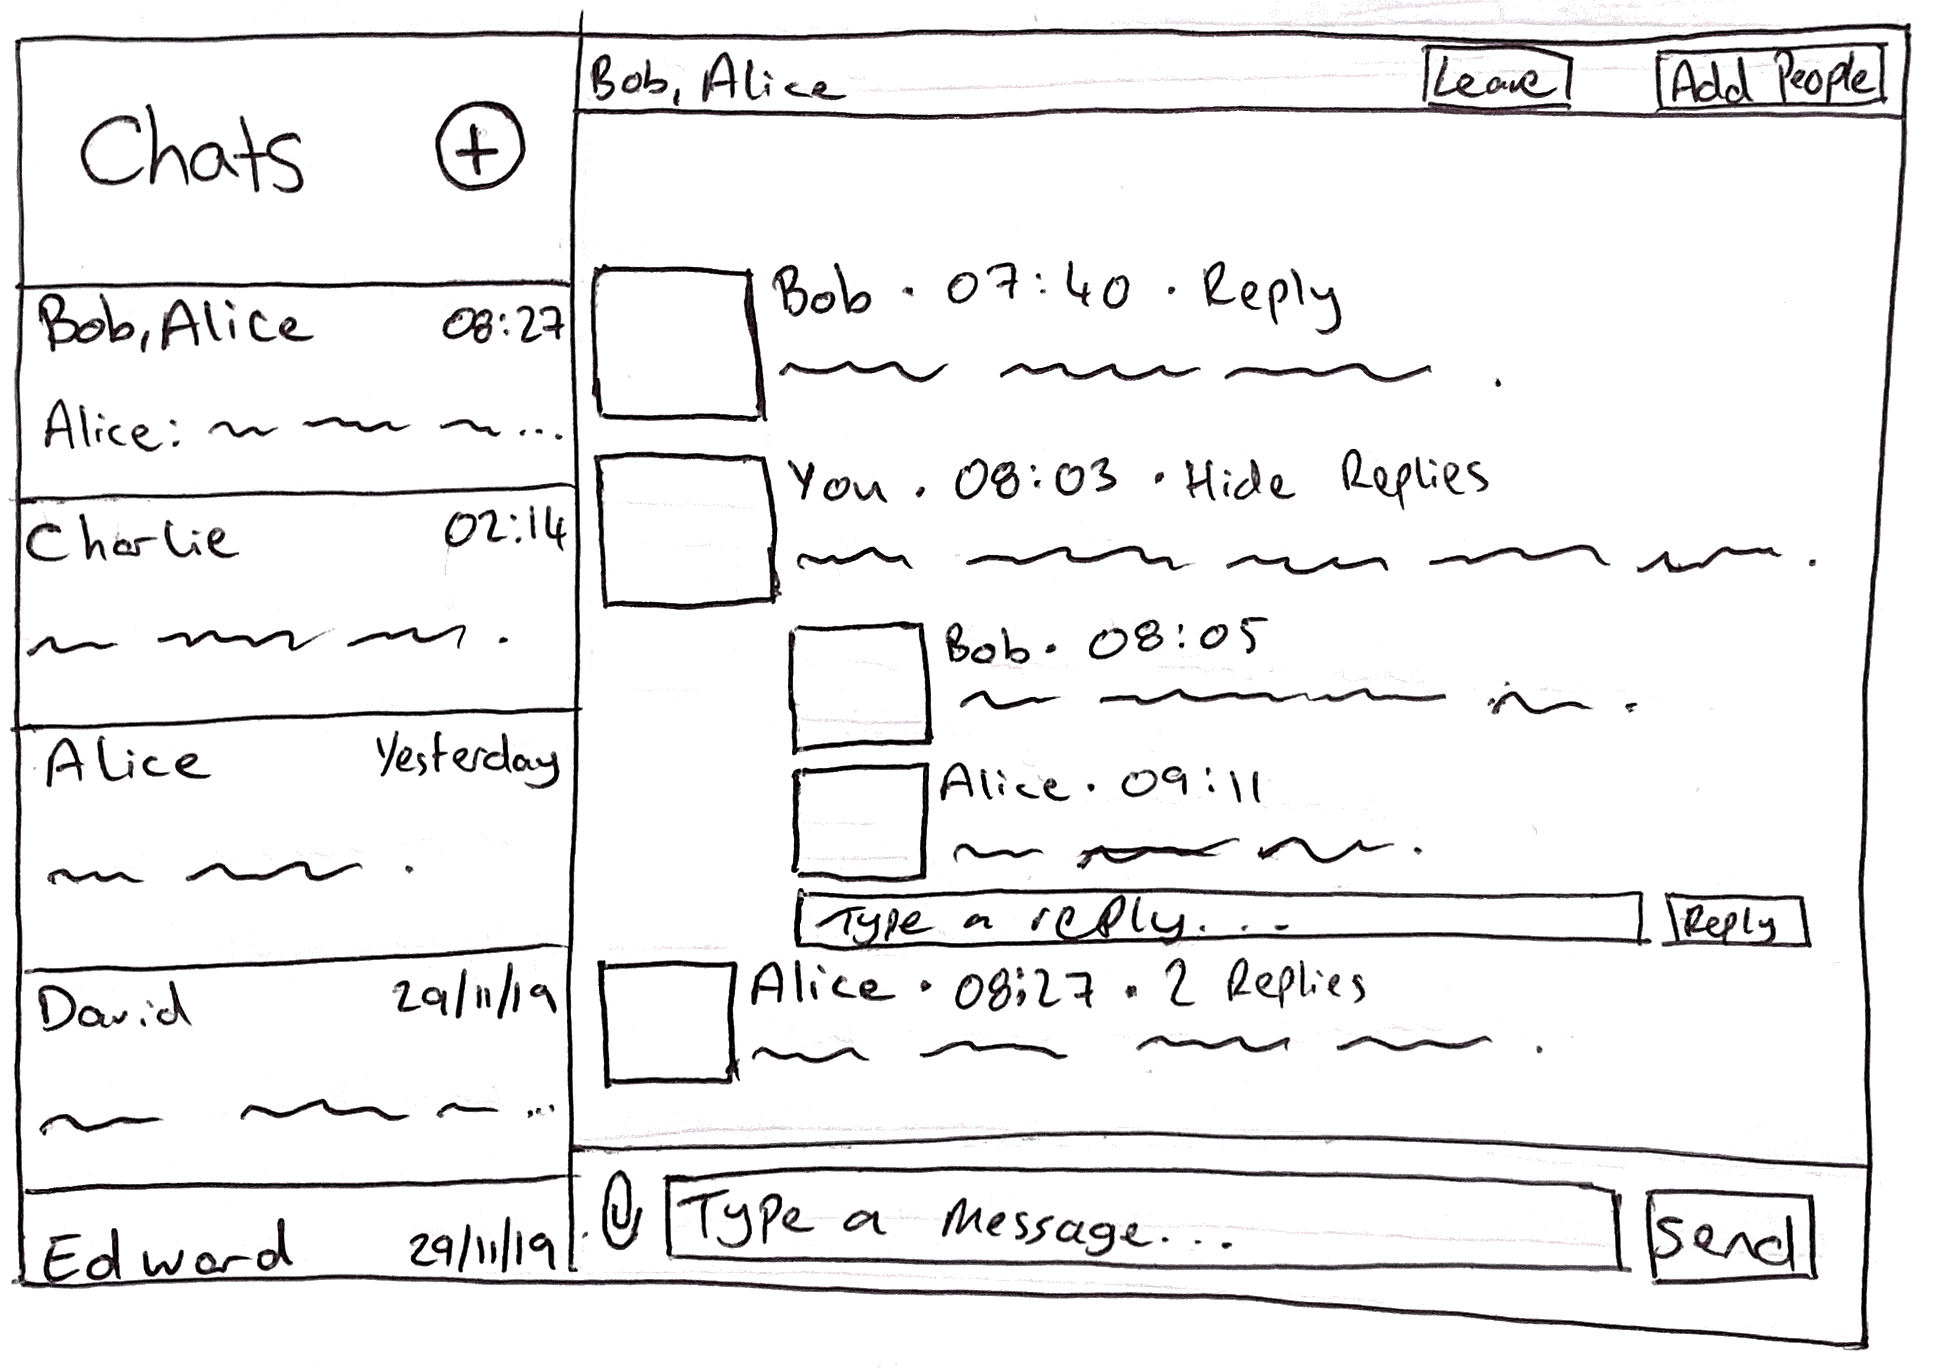
\includegraphics[width=0.8\textwidth]{images/final-design.png}
  \caption{Low-fidelity wireframe showing the main conversation screen}
  \label{fig:sketch-main} 
\end{figure}

\begin{figure}[h!]
  \centering
  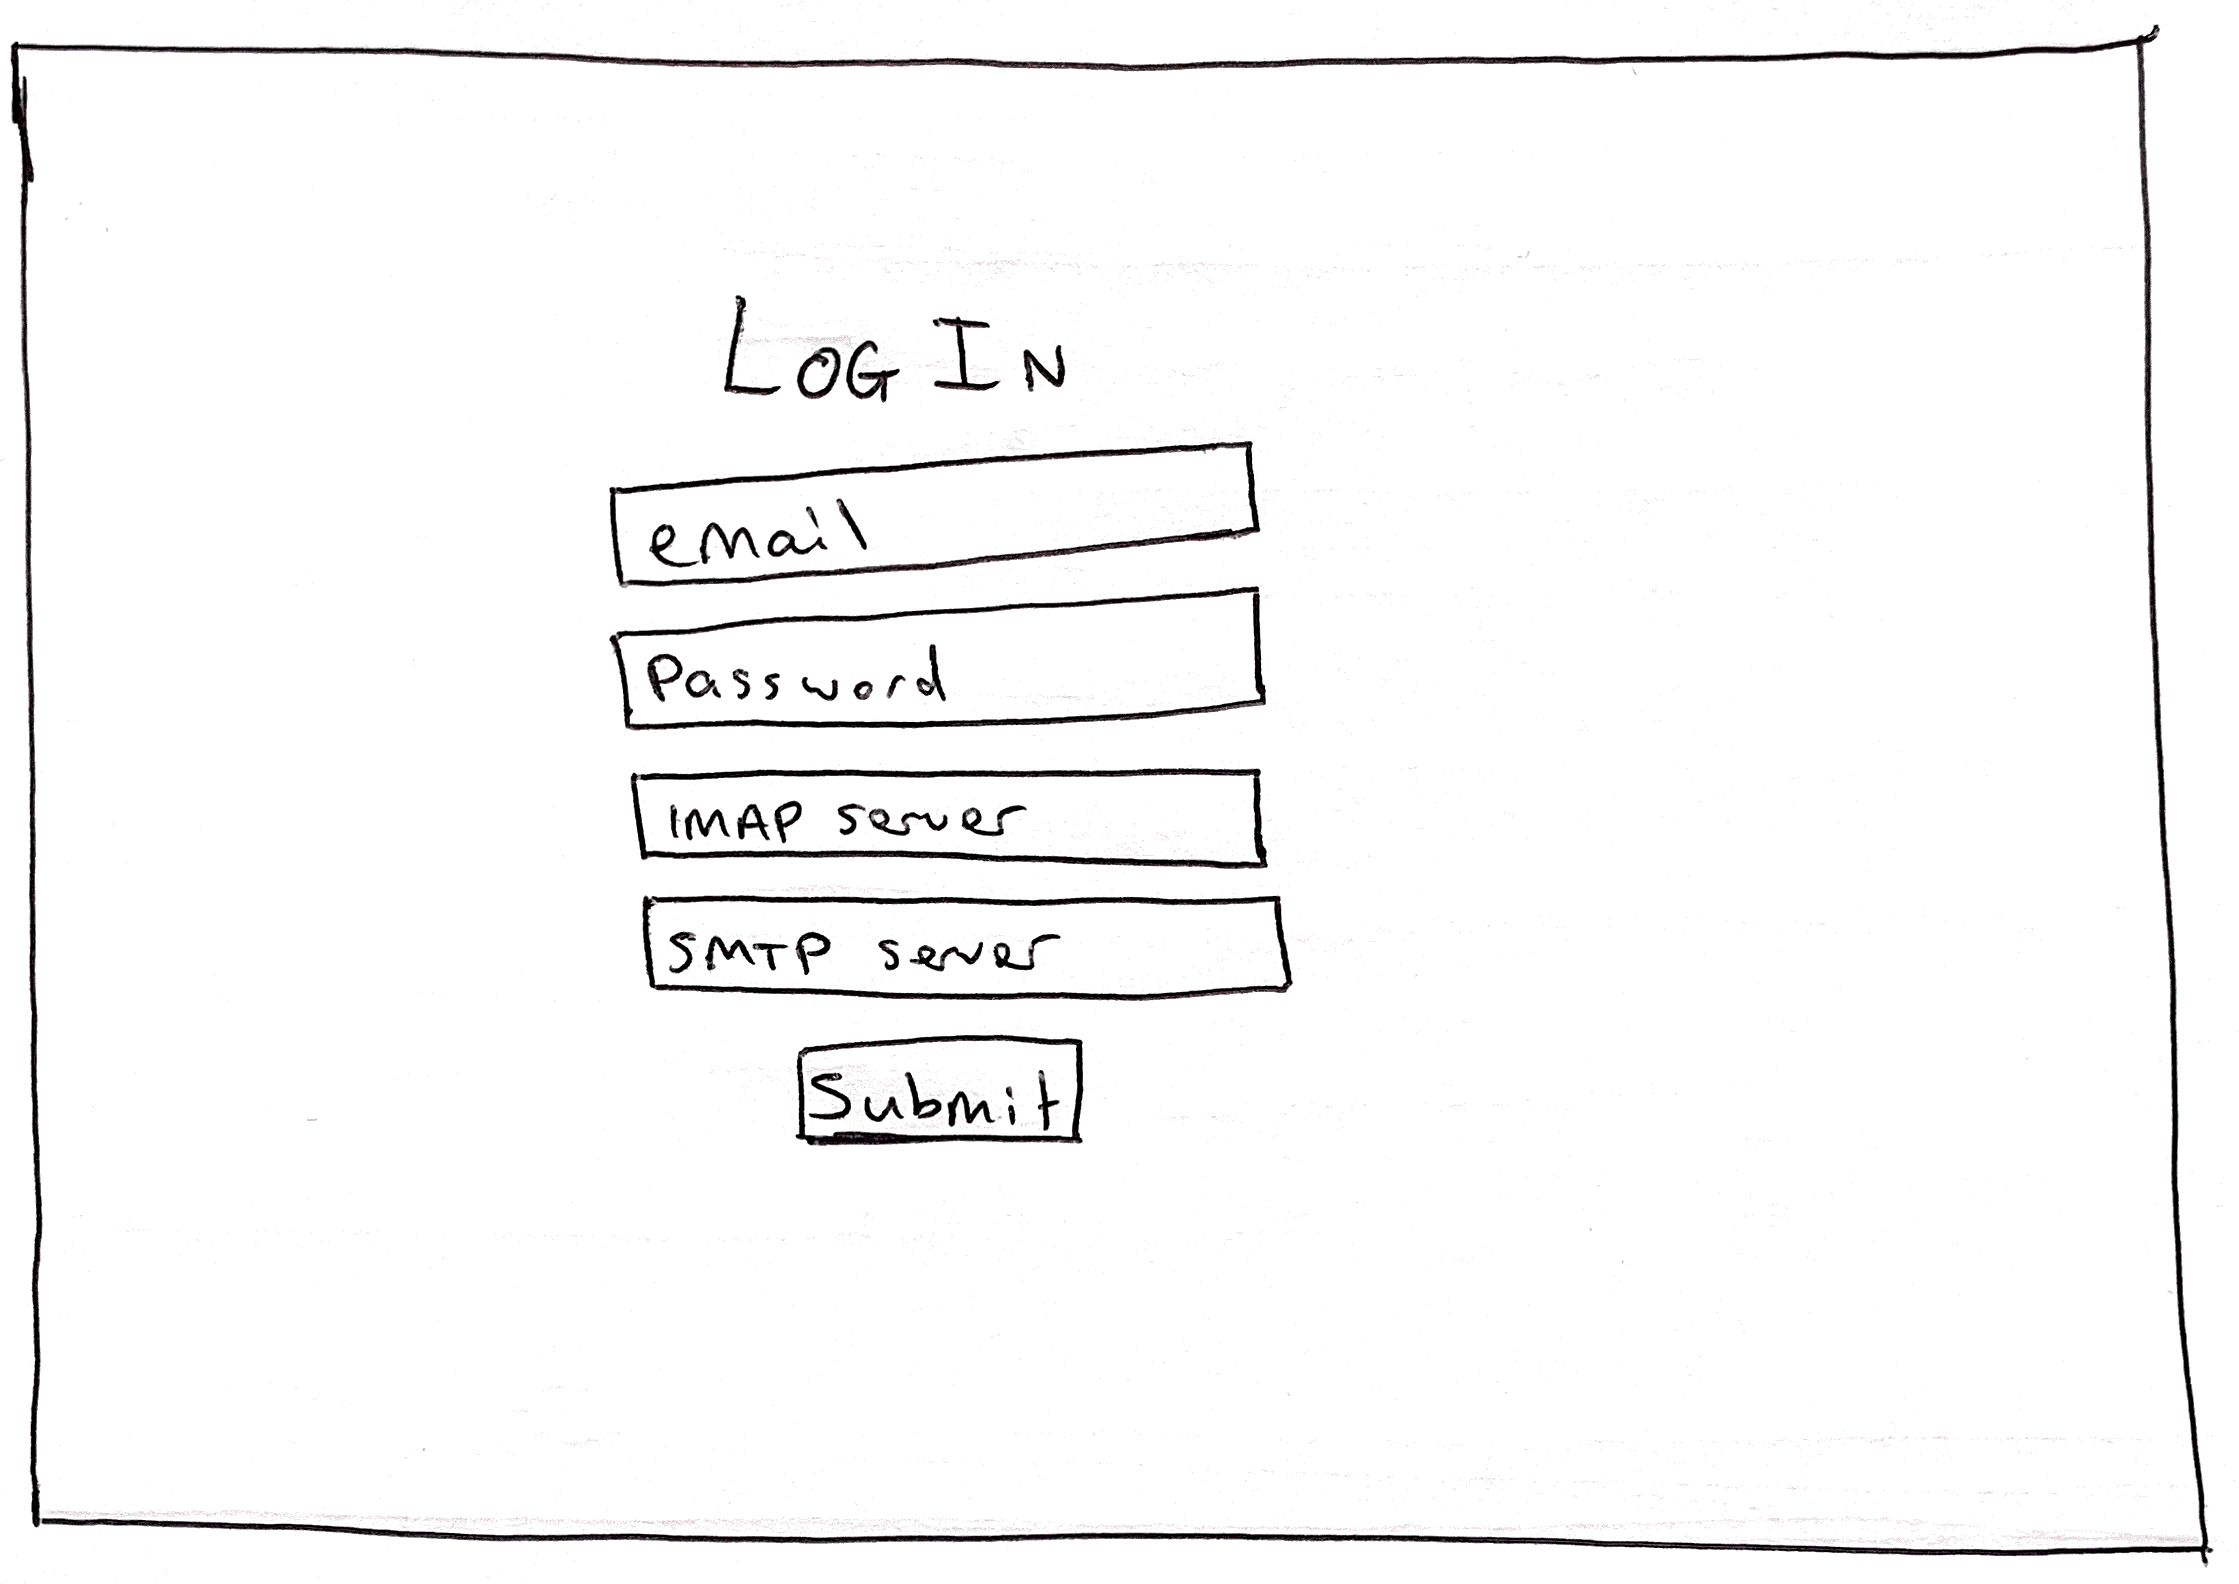
\includegraphics[width=0.8\textwidth]{images/login-design.png}
  \caption{Low-fidelity wireframe showing the login screen}
  \label{fig:sketch-login}
\end{figure}

These wireframes will be used to support building a user interface using React, however it is noted that the specifics of the design will likely change over time as the project evolves and user feedback is gathered. The designs should, however, allow for the development of a Minimum Viable Product.